\documentclass[12pt,letterpaper]{article}
\usepackage[utf8]{inputenc}
\usepackage{tikz}
\usetikzlibrary{trees}
\usepackage[spanish, es-nodecimaldot]{babel}
\usepackage{amsmath}
\usepackage{color}
\usepackage{algorithm}
\usepackage[noend]{algpseudocode}
\renewcommand{\algorithmicrequire}{\textbf{Entrada:}}
\renewcommand{\algorithmicensure}{\textbf{Salida:}}
\usepackage{subcaption}
\usepackage{amsfonts}
\usepackage{hyperref}
 \hypersetup{
     colorlinks=true,
     linkcolor=blue,
     filecolor=blue,
     citecolor = blue,      
     urlcolor=cyan,
     }
\usepackage{amssymb}
\usepackage{listings}
\usepackage{color}

\newcommand\var[1]{\, \mathrm{Var}\lbrack #1 \rbrack}

\newcommand\cov[1]{\, \mathrm{Cov} \lbrack #1 \rbrack}

\newcommand\esp[1]{\, \mathbb{E} \lbrack #1 \rbrack}

\definecolor{mygreen}{rgb}{0,0.6,0}
\definecolor{mygray}{rgb}{0.5,0.5,0.5}
\definecolor{mymauve}{rgb}{0.58,0,0.82}

\lstset{ 
  backgroundcolor=\color{white},   % choose the background color; you must add \usepackage{color} or \usepackage{xcolor}; should come as last argument
  basicstyle=\footnotesize,        % the size of the fonts that are used for the code
  breakatwhitespace=false,         % sets if automatic breaks should only happen at whitespace
  breaklines=true,                 % sets automatic line breaking
  captionpos=b,                    % sets the caption-position to bottom
  commentstyle=\color{mygreen},    % comment style
  deletekeywords={...},            % if you want to delete keywords from the given language
  escapeinside={\%*}{*)},          % if you want to add LaTeX within your code
  extendedchars=true,              % lets you use non-ASCII characters; for 8-bits encodings only, does not work with UTF-8
  firstnumber=1,                % start line enumeration with line 1000
  frame=single,	                   % adds a frame around the code
  keepspaces=true,                 % keeps spaces in text, useful for keeping indentation of code (possibly needs columns=flexible)
  keywordstyle=\color{blue},       % keyword style
  language=R,                 % the language of the code
  morekeywords={*,...},            % if you want to add more keywords to the set
  numbers=none,                    % where to put the line-numbers; possible values are (none, left, right)
  numbersep=5pt,                   % how far the line-numbers are from the code
  numberstyle=\tiny\color{mygray}, % the style that is used for the line-numbers
  rulecolor=\color{black},         % if not set, the frame-color may be changed on line-breaks within not-black text (e.g. comments (green here))
  showspaces=false,                % show spaces everywhere adding particular underscores; it overrides 'showstringspaces'
  showstringspaces=false,          % underline spaces within strings only
  showtabs=false,                  % show tabs within strings adding particular underscores
  stepnumber=2,                    % the step between two line-numbers. If it's 1, each line will be numbered
  stringstyle=\color{mymauve},     % string literal style
  tabsize=2,	                   % sets default tabsize to 2 spaces
  title=\lstname                   % show the filename of files included with \lstinputlisting; also try caption instead of title
}

\usepackage{amsthm}
\newtheorem{theorem}{Teorema}

\usepackage{graphicx}
\usepackage[inner=1.5 cm, outer = 1.5 cm, top=1 cm, bottom = 1.5 cm]{geometry}
\setlength{\parskip}{3mm}
\title{\textsc{Convolución, prueba $\chi^2$, varianza y covarianza}}
\author{\textsc{Fabiola Vázquez}}

\setlength{\parindent}{0cm}
\renewcommand{\lstlistingname}{Código}
\floatname{algorithm}{Algoritmo}
\newtheorem{ej}{Ejercicio}
\newtheorem{defi}{Definición}
\newtheorem{teo}{Teorema}

\begin{document}
\maketitle
\hrule
\section{Introducción}
El presente trabajo busca presentar resultados elementales de la varianza y covarianza de variables aleatorias. Se demuestran un par de resultados teóricos que son justificados de manera computacional. Además, se muestran aplicaciones de la técnica de convolución de funciones, y una prueba $ \chi^2 $ de bondad de ajuste.

\section{Convolución}
La convolución se aplica en el procesamiento de imágenes, específicamente cuando se desea realizar alguna transformación como podría ser la aplicación de algún filtro de difuminado o de acentuación. Para este proceso es necesario definir la convolución discreta para dos matrices \cite{fcg}, la matriz asociada a la imagen de entrada y la matriz de kernel (filtro).
\begin{defi}[Convolución discreta]
La fórmula matemática para la convolución en 2D, está dada por
\begin{equation}
\label{conv}
k[m,n] = x[m,n]*h[m,n] = \sum_{j=-\infty}^{\infty} \sum_{i=-\infty}^{\infty} x[i,j] \cdot h[m-i, n-j],
\end{equation}
donde $x$ representa la matriz de la imagen de entrada a la que se le aplica la convolución con la matriz de kernel $h$, $k$ representa la matriz de la imagen de salida. 
\end{defi}

La librería \texttt{imagine} \cite{imagine} de R \cite{R} tiene una implementación para realizar los cálculos de la convolución de matrices con la función \texttt{convolution2D}. Para ello es necesario una matriz $x$ y una matriz kernel. En el código \ref{lst:gc2} se considera una matriz $x$ de entrada de tamaño $50 \times 100$, donde los valores de las entradas de la matriz son generados con la función \texttt{runif}, la figura \ref{1} muestra la imagen asociada a dicha matriz. Como kernel se utiliza la matriz de $3 \times 3$ asociada al filtro de Gauss \cite{gauss}, es decir cuando este filtro se aplica a una imagen lo que hace es suavizarla, obteniendo una nueva imagen con difuminado.

Al realizar la convolución de la matriz \texttt{Entrada} y la matriz \texttt{Kernel}, se obtiene la matriz \texttt{Salida1}. La figura \ref{2} muestra la imagen asociada a esta matriz, como se puede ver esta es la imagen original difuminada. Si se vuelve a aplicar el filtro, pero ahora a la imagen de salida de la primera convolución se obtiene la matriz \texttt{Salida2} cuya imagen se aprecia en la figura \ref{3} la cual tiene un mayor difuminado que la figura \ref{2}.

\begin{lstlisting}[label=lst:gc2,caption=Implementación de la convolución en R., frame = single]
library("imagine")
filas    <- 50
columnas <- 100

Entrada  <- matrix(runif(filas*columnas, 0, 100), nrow = filas, ncol = columnas)
Kernel   <- matrix(c(1/16, 2/16, 1/16, 2/16, 4/16, 2/16, 1/16, 2/16, 1/16),
			      nrow=3, ncol=3)

Salida1  <- convolution2D(Entrada, kernel)
Salida2  <- convolution2D(Salida1, kernel)
\end{lstlisting}

\begin{figure}
 	\centering 
 	\begin{subfigure}[b]{0.3\linewidth}
 		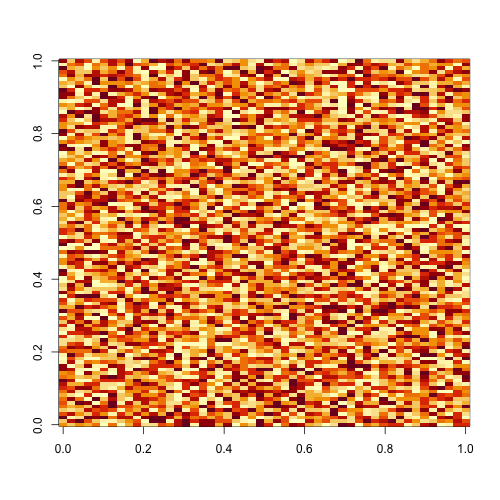
\includegraphics[width=\linewidth]{1.png} 		
 		\caption{Imagen original. \\ \, }
 		 		\label{1}
 	\end{subfigure}  \hfill
 	\begin{subfigure}[b]{0.3\linewidth}
 		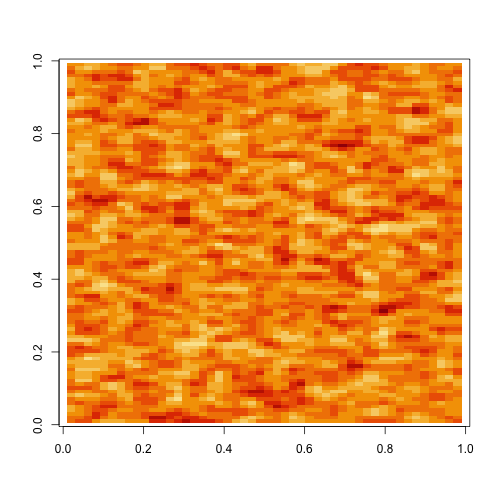
\includegraphics[width=\linewidth]{2.png} 		
 		\caption{Aplicación del filtro de Gauss a la imagen original.}
 		\label{2}
 	\end{subfigure} \hfill
 	 	\begin{subfigure}[b]{0.3\linewidth}
 		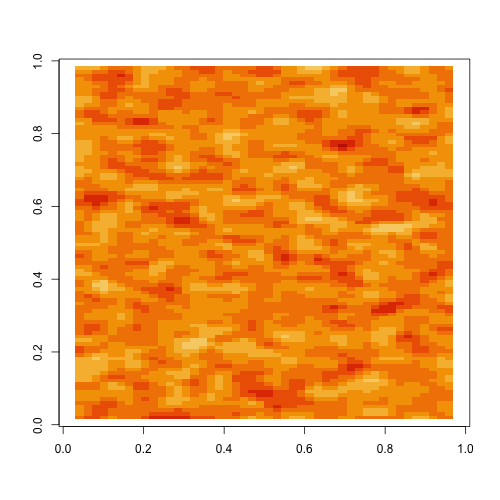
\includegraphics[width=\linewidth]{3.png} 		
 		\caption{Aplicación del filtro de Gauss a la imagen \ref{2}.}
 		\label{3}
 	\end{subfigure}
 	 	\caption{Convolución en el procesamiento de imágenes.} 
 	 		\label{im}
\end{figure}
\section{Prueba $\chi^2$}
Una de las aplicaciones de la prueba $\chi^2$ es realizar pruebas de bondad de ajuste para verificar si un conjunto de datos provienen de una población que se ajusta a un tipo de distribución de probabilidad. Como ejemplo, se trabajan con los  \href{http://jse.amstat.org/datasets/body.dat.txt}{datos} recopilados por Heinz \cite{datos}, considerando solamente la altura de las 260 mujeres.

La figura \ref{alt} muestra el histograma de los datos y por la forma de este se piensa que los datos siguen una distribución normal. Se generan 260 números con \texttt{rnorm} con media 165 y varianza 6.5, (que son la media y varianza de los datos observados). En el cuadro \ref{data} se tienen los datos observados y los esperados. Se calcula 
\begin{equation}
\sum_{1}^{10} \frac{(\text{esperado}-\text{observado})^2}{\text{esperado}}, 
\end{equation}
y se obtiene un valor aproximado de 20.83, con lo que se tiene un valor $p \approx 0.013 $, el cual es menor que 0.05, por lo que se concluye que los datos no provienen de una distribución normal.

\begin{figure}
 	\centering 
 	\begin{subfigure}[b]{0.4\linewidth}
 		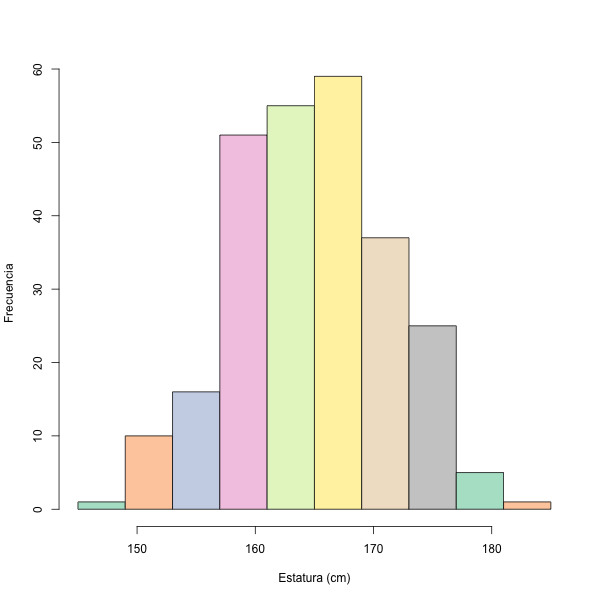
\includegraphics[width=\linewidth]{altura.png} 		
 		\caption{Histograma de las alturas de las 260 mujeres. }
 		 		\label{alt}
 	\end{subfigure}  \qquad
 	\begin{subfigure}[b]{0.4\linewidth}
 		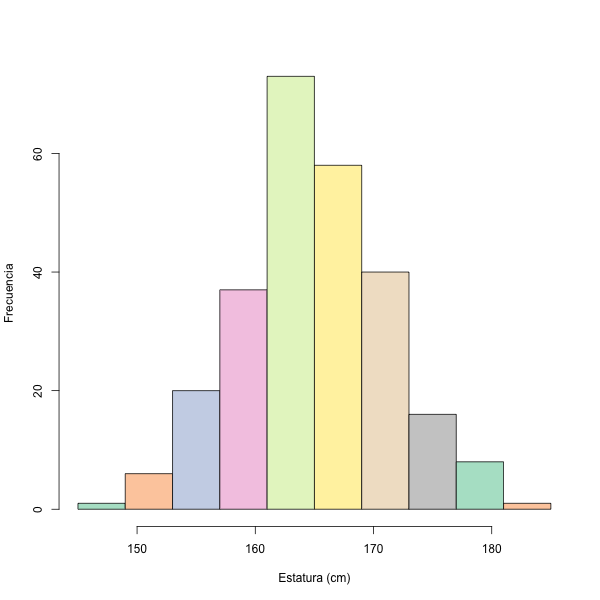
\includegraphics[width=\linewidth]{altura1.png} 		
 		\caption{Histogramas de datos generados con \texttt{rnorm(260, mean = 165, sd = 6.5)}.}
 		\label{alt1}
 	\end{subfigure}
 	 	\caption{Comparación visual de los datos observados y los datos esperados.} 
 	 		\label{im}
\end{figure}

\begin{table}
\centering
\caption{Datos observados contra los datos generados.}
\begin{tabular}{rrr}
  \hline
Estatura (cm) & Observados & Esperados \\ 
  \hline
145 - 148 & 1 & 1 \\ 
149 - 152 & 10 & 6 \\ 
153 - 156 & 16 & 20 \\ 
157 - 160 & 51 & 37 \\
161 - 164 & 55 & 73 \\
165 - 168 & 59 & 58 \\
169 - 172 & 37 & 40 \\
173 - 176 & 25 & 16 \\
177 - 180 & 5 & 8 \\
181 - 185 & 1 & 1  \\
\hline
\end{tabular}
\label{data}
\end{table}

\section{Varianza y covarianza}
Se presentan dos resultados teóricos referentes a la varianza y covarianza de dos variables aleatorias. Primeramente, se analiza dichas propiedades computacionalmente generando variables con distintas distribuciones de probabilidad y comprobando la igualdad buscada. Para cada variable aleatoria se generan 5000 números y se realizaron 100 réplicas. El cuadro \ref{teos} muestra las distribuciones generadas para las dos variables aleatorias y la cantidad de resultados en los que la igualdad es cierta, como se aprecia en dicho cuadro, de las 100 réplicas todas cumplieron la igualdad, por lo que se procede a comprobar analíticamente los teoremas. Para las demostraciones, se ocupa recordar una definición y un teorema \cite{snell} vistos anteriormente.
\begin{table}
\caption{Resultados de las pruebas computacionales.}
\begin{subtable}{0.3\textwidth}
	\centering
	\caption{Teorema 2}
	\begin{tabular}{rrr}
  \hline
$X$ &  $Y$ & Resultados\\ 
  \hline
$N(0,1)$ & $U(0,1)$ & 100 \\
$N(0,1)$ & $\text{Exp}(1)$ & 100 \\
$\text{Exp}(1)$ & $\text{Pois}(1)$ & 100 \\ 
\hline
\end{tabular}
	\label{teo1}
\end{subtable}
\hfill
\begin{subtable}{0.3\textwidth}
	\centering
	\caption{Teorema }
	\begin{tabular}{rrr}
  \hline
$X$ &  $Y$ & Resultados\\ 
  \hline
$N(0,1)$ & $U(0,1)$ & 100 \\
$N(0,1)$ & $\text{Exp}(1)$ & 100 \\
$\text{Exp}(1)$ & $\text{Pois}(2)$ & 100 \\ 
\hline
\end{tabular}
	\label{teo2}
\end{subtable}
\label{teos}
\end{table}


\begin{defi}
Sean $X$ y $Y$ variables aleatorias, se define la covarianza de $X$ y $Y$ como, 
\begin{equation}
\cov{X, Y} = \esp{XY} - \esp{X}\esp{Y}.
\end{equation}
\end{defi}

\begin{teo}
Sea $X$ una variable aleatoria, se define la varianza de $X$ como,
\begin{equation}
\var{X} = \esp{X^2} - \esp{X}^2.
\end{equation}
\end{teo}

\begin{teo}
$ \cov{aX +b, cY+d} = ac \cov{X, Y}.$
\end{teo}

\begin{proof}
\begin{align*}
 \cov{aX +b, cY+d} &= \esp{(aX+b)(cY+d)} - \esp{aX+b}\esp{cY+d} \\
&= \esp{acXY + adX + bcY +bd} - (a \esp{X} + b)(c\esp{Y}+d) \\
&= ac\esp{XY} + ad\esp{X} + bc\esp{Y} + bd - (ac\esp{X}\esp{Y} + ad\esp{X} + bc\esp{Y} + bd) \\
&= ac\esp{XY} + ad\esp{X} + bc\esp{Y} + bd - ac\esp{X}\esp{Y} - ad\esp{X} - bc\esp{Y} - bd \\
&= ac\esp{XY} - ac\esp{X}\esp{Y} \\
&=ac(\esp{XY} - \esp{X}\esp{Y}) \\
&=ac  \cov{X,Y}.
\end{align*}
\end{proof}

\begin{teo}
$\var{X+Y} = \var{X} + \var{Y} + 2 \cov{X, Y}$.
\end{teo}

\begin{proof}
\begin{align*}
\var{X+Y} &= \esp{[\left(X+Y\right)^2 - \left(\esp{X+Y}\right)^2} \\ &= E[X^2 + 2XY +Y^2] - \left(\esp{X} + \esp{Y}\right)^2 \\
&= \esp{X^2} + 2\esp{XY} + \esp{Y^2} - \esp{X}^2 - 2\esp{X}\esp{Y} - \esp{Y}^2 \\ 
&= (\esp{X^2} - \esp{X}^2) + (\esp{Y^2} - \esp{Y}^2) + 2(\esp{XY} - \esp{X}\esp{Y}) \\ 
&= \var{X} + \var{Y} + 2\cov{X, Y}.	
\end{align*}
\end{proof}
\bibliographystyle{plain} 
\bibliography{ref}


\end{document} 